\documentclass{beamer}

\useoutertheme[footline=institute,subsection=false]{miniframes}
\usecolortheme{whale}
\setbeamercolor{titlelike}{parent=structure}
\useinnertheme{rounded}

\setbeamertemplate{footline}
{%
\begin{beamercolorbox}[wd=1.0\textwidth,ht=3ex,dp=1.5ex,left,leftskip=.5em]{title in head/foot}%
\usebeamerfont{title in head/foot}%
\hspace{1em}\insertshortauthor\hfill\insertshorttitle\hfill\raggedleft\insertframenumber{} of \inserttotalframenumber\hspace{1em}
\end{beamercolorbox}%
}

\usepackage{amsmath}
\usepackage{amsfonts}
\usepackage{amssymb}
%\usepackage{bbm}
\usepackage{units}

\usepackage[final]{listings}

\newcommand{\cmd}[1]{\mbox{\small{\texttt{#1}}}}
\newcommand{\e}{\mathrm{e}}
\newcommand{\op}[1]{\hat #1}
\newcommand{\rmd}{\mathrm{d}}
\newcommand{\mean}[1]{\langle #1 \rangle}
\newcommand\T{\rule{0pt}{2.6ex}}

\renewcommand{\emph}[1]{\textbf{\color{blue}#1}}

\title[{Metaprogramming Applied to Numerical Problems}]{Metaprogramming Applied to Numerical Problems \\ {\small A Generic Implementation of Runge-Kutta Algorithms}}

\author[Mario Mulansky]{Mario Mulansky\\ Karsten Ahnert}

\date{\today} 

\institute{University of Potsdam}

\beamertemplatenavigationsymbolsempty
\titlegraphic{
\includegraphics[height=2cm]{logo.pdf}}
%\setbeamertemplate{footline}{}

\definecolor{dark-gray}{gray}{0.15}
\definecolor{light-gray}{gray}{0.8}
\definecolor{lighter-gray}{gray}{0.9}

\setbeamercolor{block title}{bg=light-gray} 
\setbeamercolor{block body}{bg=lighter-gray}

\definecolor{dark-green}{rgb}{0,0.4,0}
\definecolor{dark-red}{rgb}{0.2,0,0}

\lstset{
backgroundcolor=\color{lighter-gray},
frame=single,
basicstyle=\ttfamily\footnotesize,
tabsize=4,
keywordstyle=\color{dark-green},
identifierstyle=,
commentstyle=\color{dark-gray}\normalfont\rmfamily\itshape,
stringstyle=\color{dark-red},
language=c++,
showstringspaces=false
}


\begin{document}

\begin{frame}
\titlepage
\end{frame}

\begin{frame}{Content}

 \begin{itemize}
  \item Ordinary Differential Equations (ODEs)
  \item numerical routines: Runge-Kutta Schemes
  \item ``classic'' implementations
  \item generic implementation using Template Metaprogramming
  \item performance tests
  \item summary
 \end{itemize}
 
\end{frame}


\section{Ordinary Differential Equations}

\begin{frame}{Ordinary Differential Equations}
 ODEs are the typical way to describe physical, bioglogical, chemical, ... processes and thus play a fundamental role in mathematical modelling.
 \begin{itemize}
  \item Newton's equation of motion
  \item Reaction-diffusion systems
  \item Modelling of interacting neuronal networks
 \end{itemize}

\pause
\vspace{1em}
 Also, ODEs are used as approximations to Partial Differential Equations for numerical treatments.

\end{frame}


\begin{frame}{Ordinary Differential Equations}

 A first order ODE is written in its most general form as:
 \begin{equation}
  \frac\rmd{\rmd t} \vec{x}(t) = \vec{f}(\vec x , t )
 \end{equation} 

 \begin{itemize}
  \item $\vec x(t)$ is the function in demand (here: trajectory)
  \item $t$ is the independent variable (here: time)
  \item $f(x ,t)$ is the rhs, governing the behavior of $x$
 \end{itemize}
 
Initial Value Problem (IVP):
 \begin{equation}
  \dot x = f( x , t ) ,\qquad x(t=0) = x_0
 \end{equation} 

\end{frame}

\begin{frame}{Examples}
 \begin{itemize}
  \item $\dot x = -\lambda x$ \hspace{1cm} solution: $x(t) = x_0 \e^{-\lambda t}$
  \item $ \ddot x = \omega^2 x \rightarrow \begin{cases}\dot x = p \\ \dot p = -\omega^2 x \end{cases}$ \hspace{0cm} solution: $x(t) = A \sin(\omega t + \varphi_0)$.

\pause

  \item Lorenz System: $
\begin{aligned}
 \dot x &= \sigma ( y - x ) \\
 \dot y &= x( R - z ) - y \\
 \dot z &= xy - \beta z.
\end{aligned} $ \hspace{0.5cm} solution: ?\\
 Chaotic system (for certain parameter values $\sigma, R , \beta$), hence the solution can not be written in analytic form.
 \end{itemize}

\pause 
\vspace{1em}
$\Longrightarrow$ numerical methods to solve ODEs are required for more complicated systems.
\end{frame}


\section{Runge-Kutta Scheme}

\begin{frame}{Runge-Kutta Scheme}

One class of algorithms to solve IVP of ODEs.

\begin{itemize}
 \item Discretized time $t \rightarrow t_n = t_0 + n\cdot h$ with (small) time step $h$
 \item Trajectory $x(t) \rightarrow x_n \approx x(t_n)$
 \item Iteration along trajectory: $x_0 \longrightarrow x_1 \longrightarrow x_2 \dots$
 \item One-step method: $x_1 = \Phi(x_0)$, $x_2 = \Phi(x_1)$, $\dots$ 
\end{itemize}

\pause
\begin{center}
  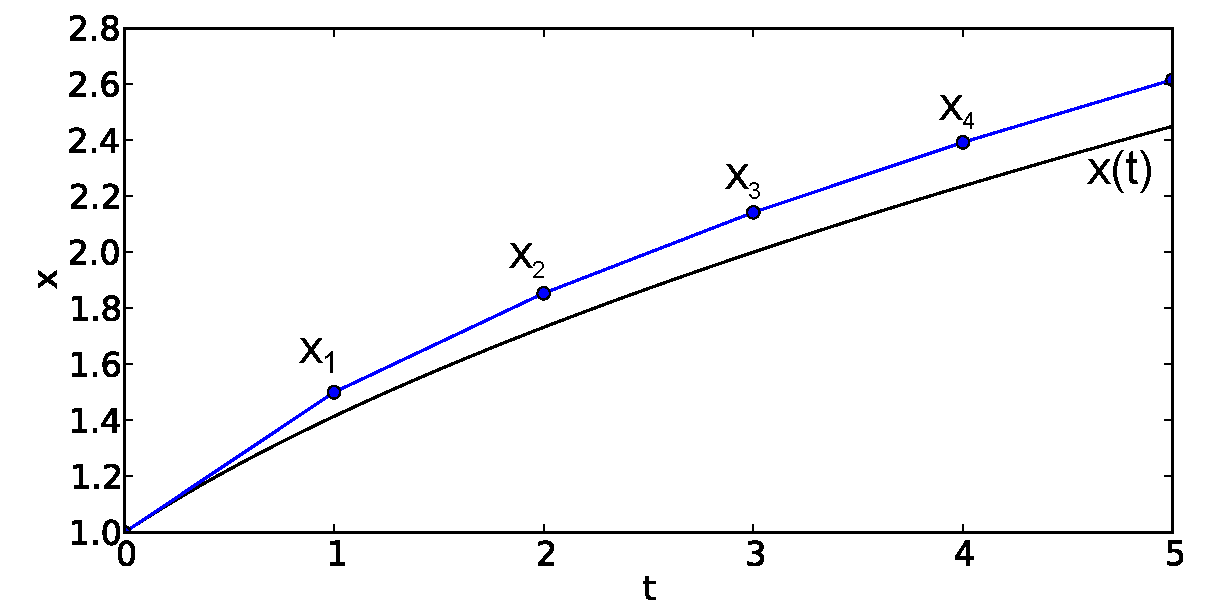
\includegraphics[width=0.8\linewidth]{x_discrete.pdf}
\end{center}

\end{frame}


\begin{frame}{Runge-Kutta Scheme}

Numerically solve the Initial Value Problem (IVP) of the ODE:
\begin{equation}
 \dot x(t) = f(x,t), \qquad x(t=0) = x_0.
\end{equation}
A Runge-Kutta scheme with $s$ stages and parameters $c_1 \dots c_s$, \hspace{.5em}$a_{21}, a_{31} , a_{32} , \dots , a_{s s-1}$ and $b_1 \dots b_s$
gives the approximate solution for $x_1 \approx x(h)$ starting at $x_0$ by computing:
\begin{equation}
 x_1 = x_0 + h\sum_{i=1}^s b_i F_i \qquad \text{where} \qquad F_i = f( x_0 + h\sum_{j=1}^{i-1} a_{ij} F_j , h c_i ).
\end{equation}

This approximate solution $x_1$ is exact up to some order $p$.

Repeating the whole procedure brings you from $x_1$ to $x_2$, then to $x_3$ and so on.

\end{frame}

\begin{frame}
 At each stage $i$ the following calculations have to be performed ($y_1 = x_0$) :
\begin{align*} \label{eqn:rk_scheme}
 F_i &= f( y_{i} , h c_i ), \qquad y_{i+1} = x_0 + h\sum_{j=1}^{i} a_{i+1,j} F_j, \qquad i=1\dots s-1\quad 
\\
 F_s &= f(y_{s} , h c_s ) , \qquad x_1 = x_0 + h\sum_{j=1}^{s} b_{j} F_j.
\end{align*}
The parameters $a$, $b$ and $c$ define the so-called Butcher tableau.

\end{frame}


\begin{frame}{Butcher Tableau}
Parameters $a$, $b$, and $c$ are typically written as Butcher tableau:

\begin{center}
 \begin{tabular}{c|ccccc}
   $c_1$ &  & & & & \\
   $c_2$ & $a_{2,1}$ & & & & \\
   $c_3$ & $a_{3,1}$ & $a_{3,2}$ & & & \\
   $\vdots$ & $\vdots$ &  & $\ddots$ & & \\
   $c_s$ & $a_{s,1}$ & $a_{s,2}$ & $\dots$ & $c_{s,s-1}$ & \\
  \hline 
    & $b_1$ & $b_2$ & $\dots$ & $b_{s-1}$ & $b_s$ \\
 \end{tabular}
\end{center}
 
The Butcher Tableau fully defines the Runge-Kutta scheme.

Each line of the tableau represents one stage of the scheme.
\end{frame}

\begin{frame}[fragile]{Explicit Non-Generic Implementation}
Given parameters \lstinline+c_i , a_ij , b_i+ 
\begin{lstlisting}
F_1 = f( x , t + c_1*dt );
x_tmp = x + dt*a_21 * F_1;

F_2 = f( x_tmp , t + c_2*dt );
x_tmp = x + dt*a_31 * F_1 + dt*a_32 * F_2;

// ...

F_s = f( x_tmp , t + c_s*dt );
x_end = x + dt*b_1 * F_1 + dt*b_2 * F_2 + ... 
          + dt*b_s * F_s; 
\end{lstlisting}

Not generic: Each stage written hard coded -- you have to adjust the algorithm when implementing a new scheme.
\end{frame}


\begin{frame}[fragile]{Run Time Implementation}
Given parameters \lstinline+a[][] , b[] , c[]+.
\begin{lstlisting}
F[0] = f( x , t + c[0]*dt );
x_tmp = x + dt*a[0][0] * F[0];

for( int i=1 ; i<s-1 ; ++i )
{
  F[i] = f( x_tmp , t + c[i]*dt );
  x_tmp = x;
  for( int j=0 ; j<i+1 : ++j )
    x_tmp += dt*a[i][j] * F[j];
}

F[s-1] = f( x_tmp , t + c[s-1]*dt );
x_end = x;
for( int j=0 ; j<s : ++j )
  x_end += dt*b[j] * F[j];
\end{lstlisting}

\pause
\textbf{Generic, but factor 2 slower than explicit implementation!}
\end{frame}


\begin{frame}[fragile]{Why Bad Performance}

The run time generic code is hard to optimize for the compiler, because:

\begin{itemize}
 \item Double \lstinline+for+ loop with inner bound depending on outer loop variable.
 \item 2D array \lstinline+double** a+ must be dynamically allocated:
\begin{lstlisting}
a = new double*[s];
for( int i=0 ; i<s ; ++i )
  a[i] = new double[i+1];
a[0][0] = ...; 
a[1][0] = ...; a[1][1] = ...; 
...
\end{lstlisting}
$\longrightarrow$ lives on heap, harder to be optimized compared to stack.
 \item Many more issues possible (optimizers are rather complex).

\end{itemize}

\end{frame}

\begin{frame}{What to do?}

\begin{block}{Idea:}
 Use template engine to generate code that can be efficiently optimized by the Compiler.
\end{block}

\vspace{1em}
\pause
More specifically, we will use Template Metaprogramming to:
\begin{itemize}
 \item Generate fixed size arrays: \lstinline+a_1[1] , a_2[2] , ... , a_s[s]+
 \item Unroll the outer \lstinline+for+-loop (over stages \lstinline+s+) so the compiler sees sequential code.
\end{itemize}

As result, the code seen by the compiler/optimizer (after resolving templates) is very close to the non-generic version and thus as fast, hopefully.
\end{frame}

\section{Generic Implementation}


\begin{frame}{Generic Runge-Kutta Algorithm}
 
\begin{Large}Idea:\end{Large}
  \begin{itemize}
    \item Write a Metaprogram that creates Runge-Kutta algorithms
    \item Metaprogram input: Parameters of the RK scheme (Butcher Tableau)
    \item Main objective: \textbf{Resulting program should be as fast as direct implementation}
  \end{itemize}

\vspace{1em}
With such a Metaprogram you can implement any new Runge-Kutta scheme by just providing the Butcher tableau.

\begin{itemize}
 \item Decrease in programming time
 \item Less bugs
 \item Better maintainability
\end{itemize}

\end{frame}


\begin{frame}[fragile]{The Generic Implementation}

Define a structure representing one stage of the Runge-Kutta scheme:

\begin{lstlisting}
template< int i >
struct stage // general (intermediate) stage, i > 0
{
  double c; // parameter c_i
  array<double,i> a; // parameters a_i+1,i ... a_i,i
                     // b_1 .. b_j for the last stage
};
\end{lstlisting}

Given an instance of this stage with \lstinline+c+ and \lstinline+a+ set appropriately the corresponding Runge-Kutta stage can be calculated. 

%\vspace{1em}
%\begin{footnotesize}Note: \lstinline+array<double,i>+ is the C++ equivalent of \lstinline+double[i]+.\end{footnotesize}
\end{frame}


\begin{frame}[fragile]{The Generic Implementation}
%Perform the calculation for this stage.
\begin{lstlisting}
// x , x_tmp , t , dt and F defined outside
template< int i >
void calc_stage( const stage< i > &stage )
{  // performs the calculation of the i-th stage
  if( i == 1 ) // first stage?
    F[i-1] = f( x , t + stage.c * dt );
  else
    F[i-1] = f( x_tmp , t + stage.c * dt );

  if( i < s ) { // intermediate stage?
    x_tmp = x;
    for( int j=0 ; j<i : ++j )
      x_tmp += dt*stage.a[j] * F[j];
  } else {   // last stage
    x_end = x;
    for( int j=0 ; j<i : ++j )
      x_end += dt*stage.a[j] * F[j];
  }
}
\end{lstlisting}
\end{frame}

\begin{frame}[fragile]{The Generic Implementation}
Generate list of stage types: \lstinline+stage<1> , stage<2>, ... , stage<s>+ using Boost.MPL (MetaProgramming Library) and Boost.Fusion.

\begin{lstlisting}[basicstyle=\ttfamily\tiny]
typedef mpl::range_c< int , 1 , s > stage_indices;

typedef typename fusion::result_of::as_vector
< typename mpl::push_back
  < typename mpl::copy
    < stage_indices,
      mpl::inserter
      <
        mpl::vector0<> ,
        mpl::push_back< mpl::_1 , stage_wrapper< mpl::_2 , stage > >
      >
    >::type , stage< double , stage_count , last_stage >
  >::type
>::type stage_vector_base; //fusion::vector< stage<1> , stage<2> , ... , stage<s>

struct stage_vector : stage_vector_base
{
  // initializer methods
  stage_vector( const a_type &a , const b_type &b , const c_type &c )
  {
    // ...
  }
}
\end{lstlisting}

\end{frame}

\begin{frame}[fragile]{The Generic Implementation}
Parameter types for \lstinline+a+, \lstinline+b+ and \lstinline+c+:
\begin{lstlisting}[basicstyle=\ttfamily\tiny]
typedef typename fusion::result_of::as_vector
< typename mpl::copy
  < stage_indices ,
    mpl::inserter
    < mpl::vector0< > ,
      mpl::push_back< mpl::_1 , 
                      array_wrapper< double , mpl::_2 > >
    >
  >::type
>::type a_type; //fusion::vector< array<double,1> , array<double,2> , ... >

typedef array< double , s > b_type;
typedef array< double , s > c_type;
\end{lstlisting}

\pause
Instead of a dynamically allocated \lstinline+double**+ the compiler/optimzier sees fixed size arrays: \lstinline+array<double,1>+ , \lstinline+array<double,2>+, ... \\
$\longrightarrow$ \textbf{better optimization possibilities}
\end{frame}

\begin{frame}[fragile]{The Generic Implementation}
The actual Runge-Kutta step (details ommited):
\begin{lstlisting}[basicstyle=\ttfamily\tiny]
fusion::for_each( stages , 
                  calc_stage_caller( f , x , x_tmp , x_end , F , t , dt ) );
\end{lstlisting}
Remember: \lstinline+stages+ is \lstinline+fusion::vector< stage<1> , stage<2> , ... >+
For each of the \lstinline+stages+, \lstinline+calc_stage+ gets called, but the \lstinline+for_each+-loop is \textbf{executed by the compiler!}

\pause
\vspace{1em}
The compiler/optimizer sees sequential code:
\begin{lstlisting}
calc_stage( stage_1 ); // stage_1 is an 
calc_stage( stage_2 ); // instance of stage<1>
...                    // similar for stage_2 ...
calc_stage( stage_s );
\end{lstlisting}

$\longrightarrow$ \textbf{better optimization possibilities}

\end{frame}


\begin{frame}[fragile]{The Generic Stepper}
Provide some handy interface to the generic algorithm:
 \begin{lstlisting}[basicstyle=\ttfamily\tiny]
template< int s >
class generic_runge_kutta
{
public:
  generic_runge_kutta( const coef_a_type &a ,
                       const coef_b_type &b ,
                       const coef_c_type &c )
    : m_stages( a , b , c )
  { }

  void do_step( System f , const state_type &x , const double t , 
                state_type &x_out , const double dt )
  {
    fusion::for_each( m_stages , calc_stage_caller( f , x , m_x_tmp , x_out , 
                                                    m_F , t , dt ) );
  }

private:
  stage_vector m_stages;
  state_type m_x_tmp;

protected:
  state_type m_F[s];
};
\end{lstlisting}

\end{frame}


\section{Performance}

\begin{frame}[fragile]{Example: Runge-Kutta 4}

\begin{center}
Butcher Tableau: 
 \begin{tabular}{c|cccc}
   0 &  & &  & \\
   0.5 & 0.5 & & & \\
   0.5 & 0 & 0.5 & & \\
   1.0 & 0 & 0 & 1.0 & \\
  \hline 
    & 1/6 & 1/3 & 1/3 & 1/6 \\
 \end{tabular}
\end{center}


\begin{lstlisting}[basicstyle=\ttfamily\scriptsize]
 // define the butcher array
const array< double , 1 > a1 = {{ 0.5 }};
const array< double , 2 > a2 = {{ 0.0 , 0.5 }};
const array< double , 3 > a3 = {{ 0.0 , 0.0 , 1.0 }};

const a_type a = fusion::make_vector( a1 , a2 , a3 );
const b_type b = {{ 1.0/6.0 , 1.0/3.0 , 1.0/3.0 , 1.0/6.0 }};
const c_type c = {{ 0.0 , 0.5 , 0.5 , 1.0 }};

// create the stages with the rk4 parameters a,b,c
generic_runge_kutta< 4 > rk4( a , b , c );
// do one rk4 step
rk4.do_step( lorenz , x , 0.0 , x , 0.1 ); 
\end{lstlisting}
\end{frame}


\begin{frame}{Performance}
Did we achieve our aim? Test RK4 on Lorenz System!

\pause
%\vspace{1em}
\begin{columns}
\begin{column}{0.55\linewidth}
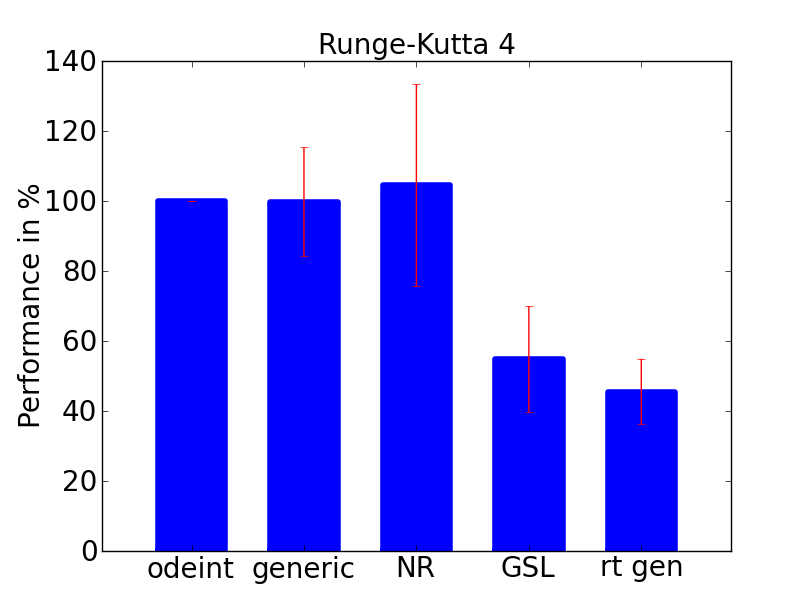
\includegraphics[width=1.0\linewidth]{perf_rk4.png}
\end{column}
\begin{column}{0.4\linewidth}
\begin{scriptsize}
  \begin{tabular}[b]{c}
    \textbf{Processors:} \\
    Intel Core i7 830 \\
    Intel Core i7 930 \\
    Intel Xeon X5650 \\
    Intel Core2Quad Q9550 \\
    AMD Opteron 2224 \\
    AMD PhenomII X4 945 \\
    \hline
    \textbf{Compilers:} \\
    gcc 4.3 , 4.4 , 4.5 , 4.6 \\
    intel icc 11.1 , 12.0 \\
    msvc 9.0
  \end{tabular}               
\end{scriptsize}
\end{column}
\end{columns}

\pause
\begin{center}
\textbf{Yes!}
\end{center}
\pause%
\begin{small}
\begin{itemize}
\item On modern compilers (Intel 12, gcc 4.5/4.6) as fast as explicit code.
\item Older compilers might produce slightly worse performant code.
\item Always factor 2 better than run time generic implementation.
\end{itemize}
\end{small}

\end{frame}

\begin{frame}{Performace}
 Second test with a different scheme: Runge-Kutta Cash-Karp 5(4)
 \begin{center} 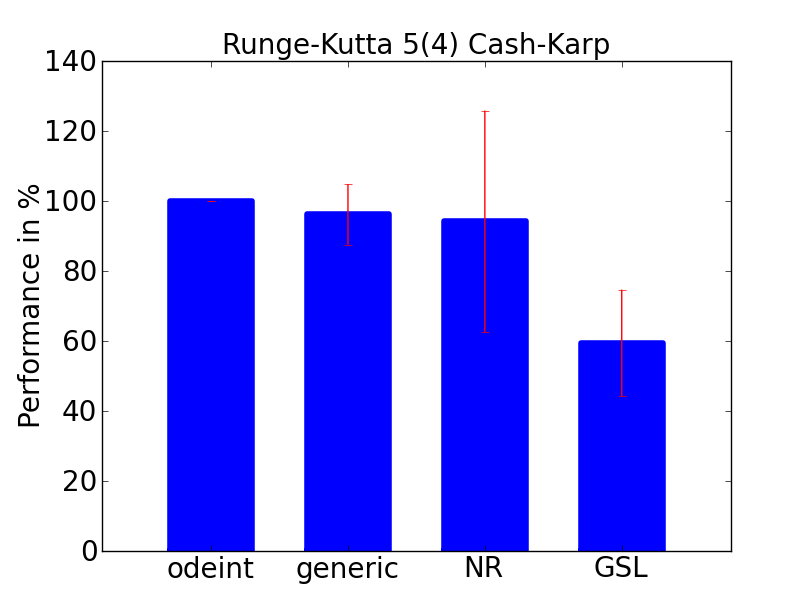
\includegraphics[width=0.8\linewidth]{perf_rk54ck.png} \end{center}
\end{frame}


\begin{frame}{Conclusions}
We implemented a generic Runge-Kutta algorithm that executes \textbf{any} RK scheme and has the following properties:
\begin{itemize}
 \item Parameters (Butcher Tableau) can be defined in a natural way as C++ Arrays
 \item By virtue of Template Metaprogramming our code is as fast as direct implementation of the specific scheme
 \item \textbf{Major improvement (factor 2) compared to generic run time implementation} (but some increase in compile time)
 \item Embedded methods with error estimate can also be easily covered in a generic way
 \item This technique can be applied to other numerical problems, e.g.\ spline fitting, ...
\end{itemize}

\pause
\vspace{1em}
\begin{center}
 \begin{huge}Thank you\end{huge}
\end{center}

\end{frame}


\begin{frame}
 

\begin{center}
\huge
 www.odeint.com
\end{center}

\end{frame}


\end{document}